\chapter{Komunikasi Perangkat Keras}

\section{Pemahaman Teori}

\subsection{Apa itu /dev pada linux}
/dev pada linux merupakan sebuah lokasi device. Jadi, jika kita ingin mengetahui lokasi device yang terhubung ke pc/laptop kita dapat mengeceknya lewat /dev.

\subsection{Installasi Driver Arduino Linux (Ubuntu 19.10)}
Untuk melakukan installasi arduino pada linux cukup mudah hampir sama seperti menggunakan windows yaitu : 
\begin{enumerate}
\item Download filenya terlebih dahulu dengan mengunjungi website arduino.
\begin{figure}[H]
\centering
\caption{Download Arduino}
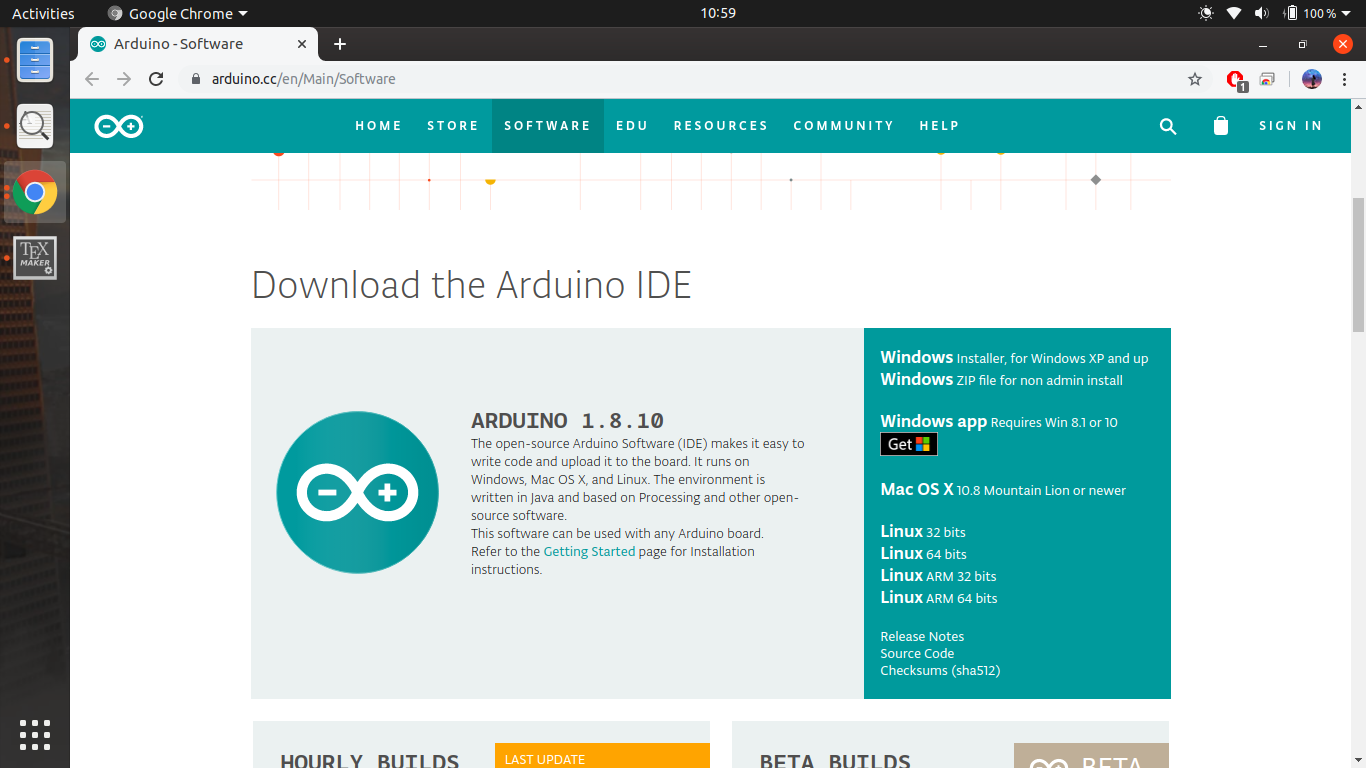
\includegraphics[width=1\textwidth]{figures/1.png}
\label{downloadarduinosoftware}
\end{figure}

\item Setelah di download kita ekstrak filenya.
\begin{figure}[H]
\centering
\caption{Ekstrak File}
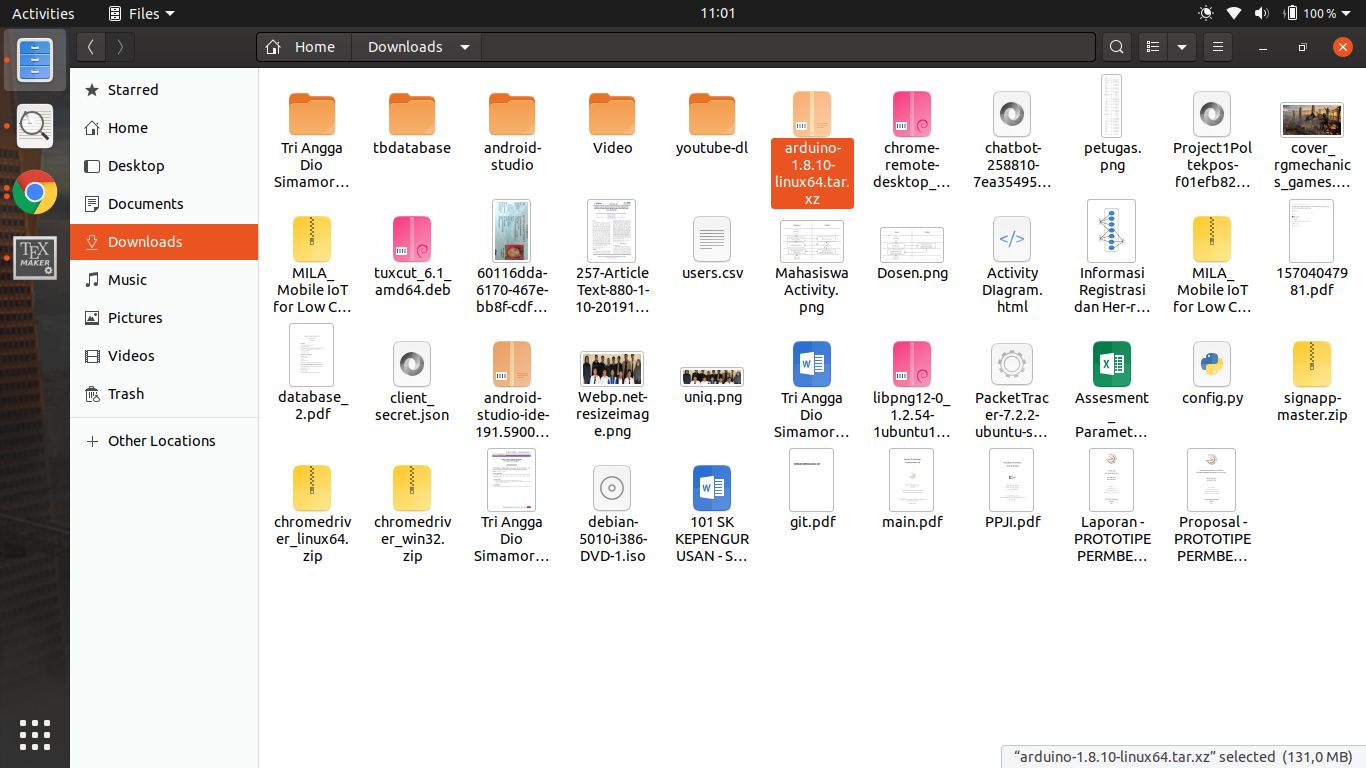
\includegraphics[width=1\textwidth]{figures/2.png}
\label{ekstrakfilearduino}
\end{figure}

\item Lalu kita masuk ke folder hasil ekstraknya
\begin{figure}[H]
\centering
\caption{Masuk Ke Folder Hasil Ekstrak}
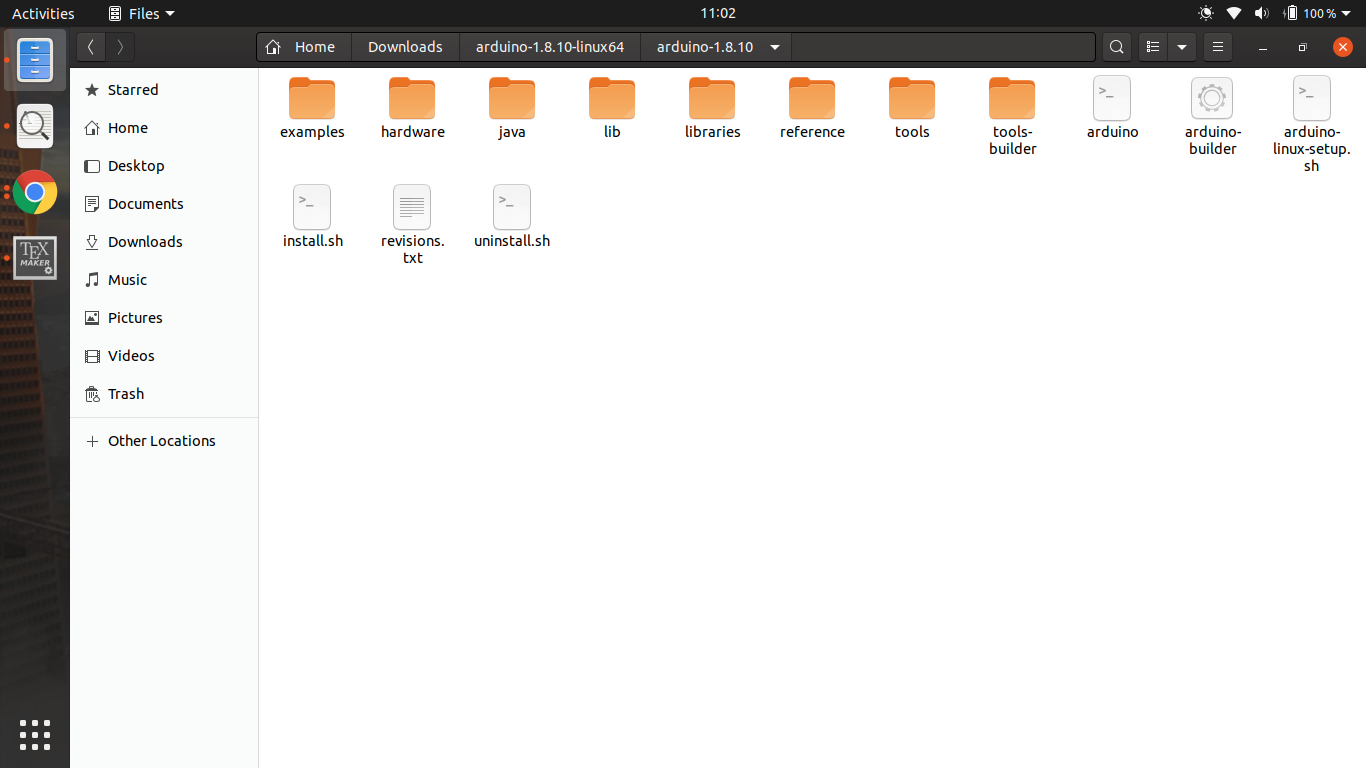
\includegraphics[width=1\textwidth]{figures/3.png}
\label{masukfolderarduino}
\end{figure}

\item Setelah itu kita buka terminal dengan cara klik kanan lalu open terminal.
\begin{figure}[H]
\centering
\caption{Buka Terminal}
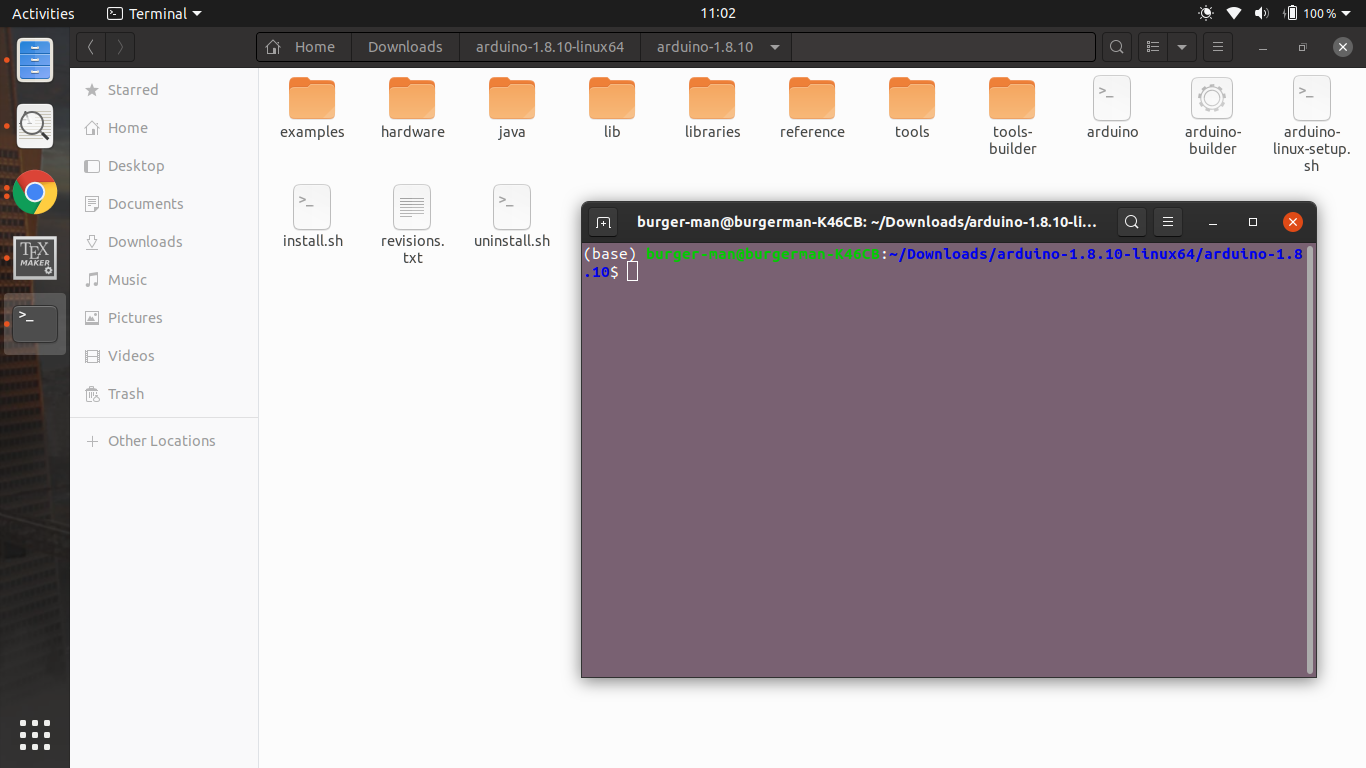
\includegraphics[width=1\textwidth]{figures/4.png}
\label{bukaterminal}
\end{figure}

\item Lalu ketikkan, \textit{sudo ./install.sh}
\begin{figure}[H]
\centering
\caption{Install Arduino}
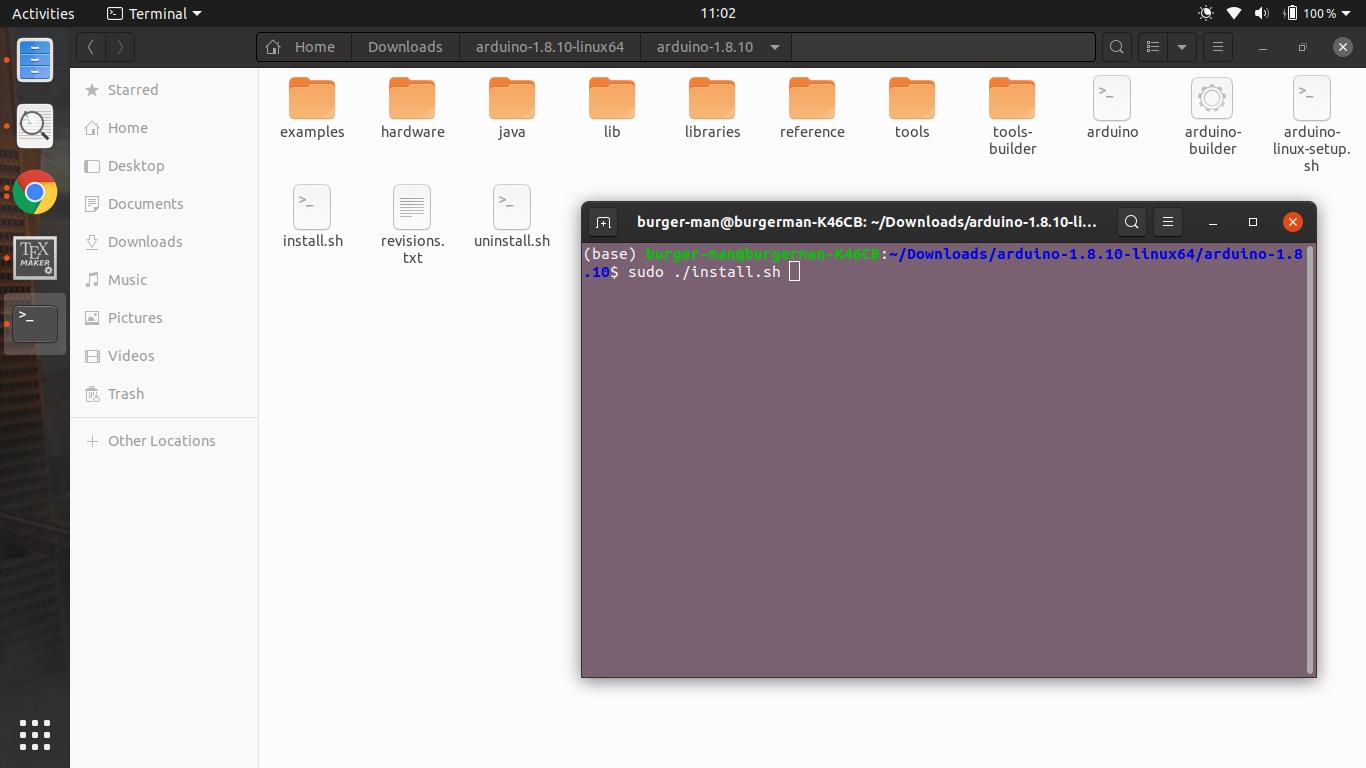
\includegraphics[width=1\textwidth]{figures/5.png}
\label{installarduino}
\end{figure}

\item Lalu, tunggu hingga muncul tulisan done.
\begin{figure}[H]
\centering
\caption{Done!}
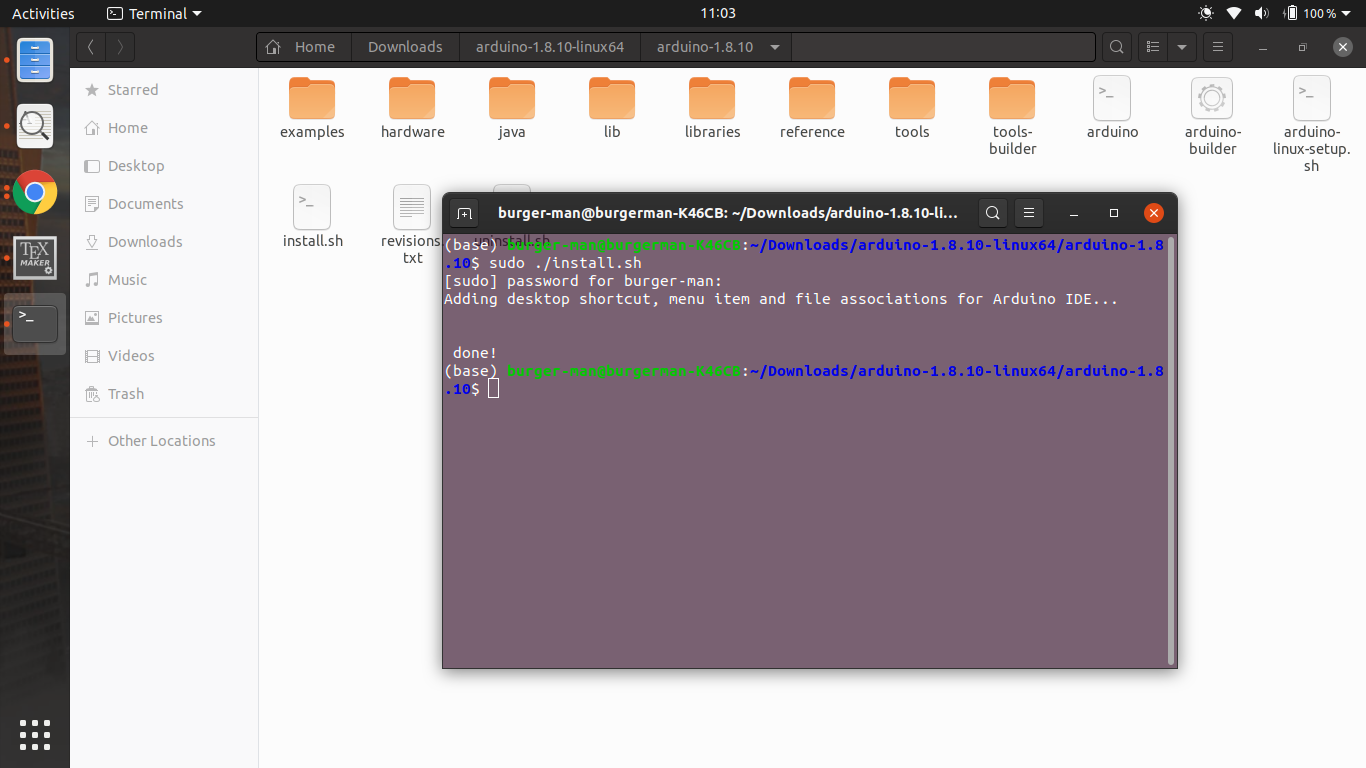
\includegraphics[width=1\textwidth]{figures/6.png}
\label{tungguselesai}
\end{figure}

\item Arduino siap digunakan
\begin{figure}[H]
\centering
\caption{Arduino}
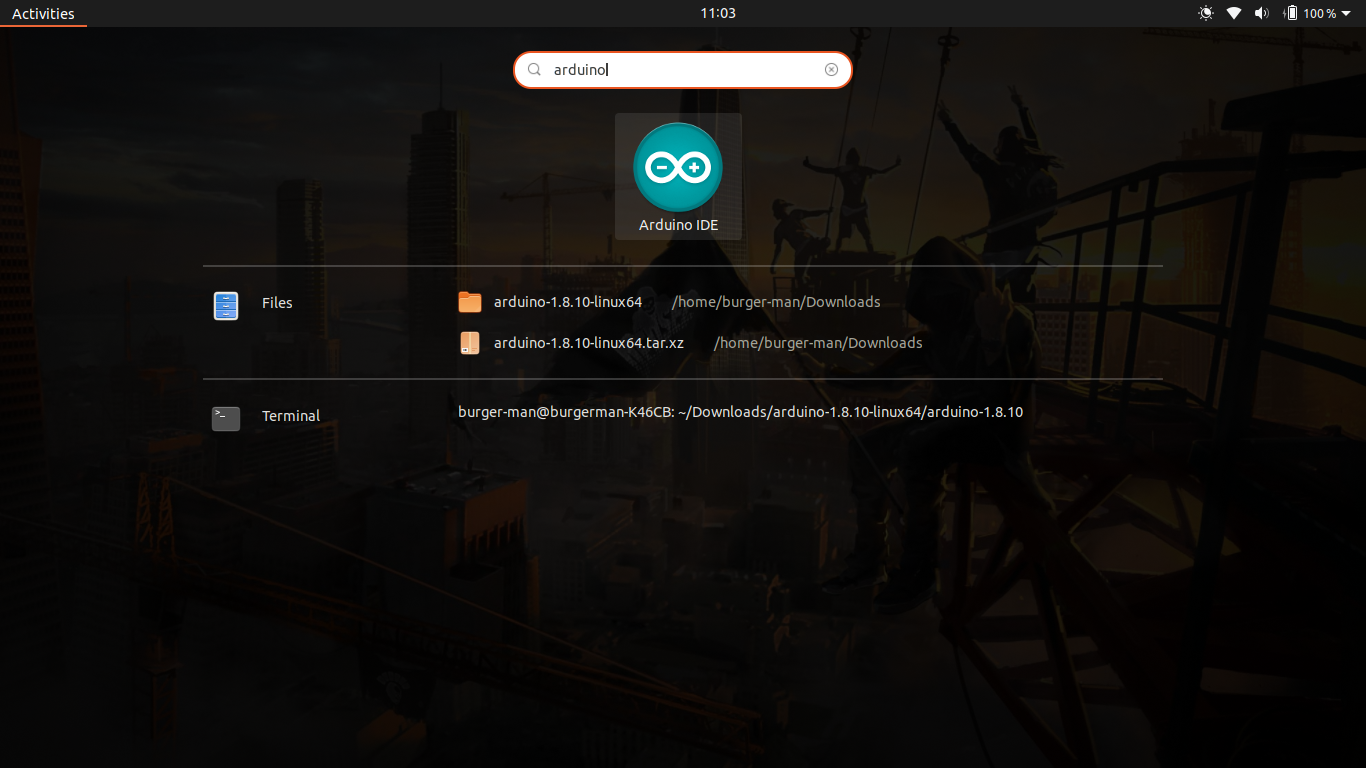
\includegraphics[width=1\textwidth]{figures/7.png}
\label{arduino}
\end{figure}
\end{enumerate}

\subsection{Baudrate dan Port}
Cara membaca baudrate cukup mudah yaitu kita lihat berapa baudrate yang digunakan misalnya kita menggunakan maximum baudrate dari arduino yaitu 115.2k (115200) satuan dari baudrate adalah bps (bit-per second) artinya ada 115200 bit dalam satu detik. sehingga misalnya jika arduino menerima 200000 maka arduino dapat menerima semua data tersebut kurang/lebih dua detik. Lalu gambar \ref{portarduino} muncul port arduino yang disambungkan ke laptop melalui USB dan dikenali dengan nama \textit{ttyACM0}

\begin{figure}
\centering
\caption{Port Arduino}

\includegraphics[width=1\textwidth]{figures/8.png}
\label{portarduino}
\end{figure}

\subsection{pyserial}
Pyserial pertama kali dirilis tahun 2001 oleh Chris Liechti. Library ini digunakan untuk mengakses serial port atau berkomunikasi pada sebuah hardware dengan bahasa pemrograman Python.